\documentclass[12pt]{scrreprt}  
% Use scrreprt class for reports

%Font Selection
% \usepackage{fontspec}
% \usepackage{times}
% \usepackage{palatino}
% \usepackage{charter}
% \setmainfont{Georgia}
% \setmainfont{Arial}


\usepackage{fontspec}
\setmainfont{Times New Roman}

\usepackage{charter}

\usepackage{graphicx}
\usepackage{array} % For better column control
\usepackage[numbers]{natbib}  % Use natbib for controlling citations
\setlength{\tabcolsep}{12pt}  % Adjusts the padding of the table cells
\renewcommand{\arraystretch}{1.5}  % Adjusts the vertical padding (row height)

% Encoding and languages
\usepackage[utf8]{inputenc}
\usepackage[english]{babel}

% Geometry and page setup
\usepackage[a4paper, margin=1in]{geometry}
\usepackage{float}


\usepackage[utf8]{inputenc}
\usepackage[english]{babel}
\usepackage{hyperref}

% Better handling of URLs and hyperlinks
\usepackage{hyperref}

% Code listings
\usepackage{listings}

% Table management
\usepackage{booktabs}
\usepackage[table,xcdraw]{xcolor}

% Flowchart and diagrams
\usepackage{tikz} 
\usetikzlibrary{shapes, arrows.meta, positioning, backgrounds}

% For easier formatting of captions
\usepackage[justification=centering]{caption}

% For defining acronyms
\usepackage[acronym]{glossaries}

% For rotating tables or figures
\usepackage{rotating}

% SI units handling
\usepackage{siunitx}

% Array handling
\usepackage{array}

% Fancy counters
\usepackage{chngcntr}

% Define styles for different node types
\tikzstyle{startstop} = [rectangle, rounded corners, minimum width=3cm, minimum height=1cm, text centered, draw=black, fill=red!30]
\tikzstyle{process} = [rectangle, minimum width=3.5cm, minimum height=1cm, text centered, draw=black, fill=blue!10]
\tikzstyle{database} = [rectangle, minimum width=3cm, minimum height=1cm, text centered, draw=black, fill=orange!30]
\tikzstyle{auth} = [rectangle, minimum width=3cm, minimum height=1cm, text centered, draw=black, fill=green!30]
\tikzstyle{ui} = [rectangle, minimum width=3.5cm, minimum height=1cm, text centered, draw=black, fill=yellow!30]
\tikzstyle{arrow} = [thick,->,>=stealth]

% For stickman (used in diagrams)
\tikzset{
    stickman/.pic={
        % Head
        \draw[fill=gray] (0,0.6) circle (0.3cm);
        % Body
        \draw[line width=0.5mm] (0,0.3) -- (0,-0.6);
        % Arms
        \draw[line width=0.5mm] (-0.4,0.3) -- (0.4,0.3);
        % Legs
        \draw[line width=0.5mm] (0,-0.6) -- (-0.4,-1.2);
        \draw[line width=0.5mm] (0,-0.6) -- (0.4,-1.2);
    }
}

\hypersetup{
    bookmarks=true,    % show bookmarks bar
    pdftitle={Software Requirement Specification}, % title
    pdfauthor={Jean-Philippe Eisenbarth},         % author
    pdfsubject={TeX and LaTeX},                    % subject of the document
    pdfkeywords={TeX, LaTeX, graphics, images},    % list of keywords
    colorlinks=true,                               % colored links
    linkcolor=blue,                                % color of internal links
    citecolor=black,                               % color of links to bibliography
    filecolor=black,                               % color of file links
    urlcolor=purple,                               % color of external links
    linktoc=page                                   % only page is linked
}


\title{Project proposal format For B.Sc. CSIT/BIT, TU, IOST}
\author{Prakash Neupane}
\date{\today}

\begin{document}
\pagenumbering{roman} % Roman page numbers

\addcontentsline{toc}{section}{TITLE PAGE}
\thispagestyle{empty} % This will hide the page number on the title page
\begin{titlepage}
    \centering
    \begin{center}
        \includegraphics[width=0.3\textwidth]{./Images/PUClogo.png} % Adjust width as necessary
    \end{center}
\begin{center}
    \textbf{Department of Computer Science and Engineering}\\
    Premier University
\end{center}
\begin{center}
    \textnormal{ CSE 338: Software Development }
\end{center}
    \vspace{0.5in}
    \small
    \textbf{A Project Proposal Report On}\\
    \vspace{0.5in}
    \large
    \uppercase{\textbf{Odyssey Travel Agency Software}}\\
    \vspace{0.5in}
    \large
    \textbf {Submitted by}\\
    \begin{center}
        \renewcommand{\arraystretch}{1.5} % Adjusts vertical spacing in the table
        \begin{tabular}{|>{\raggedright\arraybackslash}p{0.6\textwidth}|p{0.3\textwidth}|} % Adjust column widths
        \hline
        \textbf{Name} & \textbf{ID} \\
        \hline
        Mohammad Hafizur Rahman Sakib & 0222210005101118 \\
        \hline
        Arnab Shikder & 0222210005101098 \\
        \hline
        Sayed Hossain & 0222210005101102 \\
        \hline
        Mohammad Asmual Hoque Yousha & 0222210005101121 \\
        \hline
        \end{tabular}
        \end{center}
    \vspace{0.5in}
 
\begin{minipage}[t]{0.5\textwidth}
        \textbf{Submitted to :}
        \\Tashin Hossain
        \\Lecturer,Department of CSE
        \\ Premier University
        \\ Chittagong
    \end{minipage}%
    \begin{minipage}[t]{0.6\textwidth}
        \raggedleft
        \textbf{Remarks}\\
        \vspace{0.5cm} % Adjust vertical space for remarks
        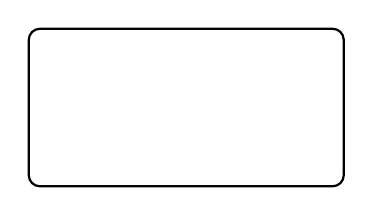
\begin{tikzpicture}
            \draw[thick, rounded corners] (0,0) rectangle (4,2);
        \end{tikzpicture}
    \end{minipage}

    \date{\today}
    \vfill
\end{titlepage}


\newpage % Ensure this file exists and is correctly formatted

% Table of contents
\newpage
{
  \setlength{\parskip}{0em}
  \renewcommand\contentsname{TABLE OF CONTENTS} % This will change heading text
  \tableofcontents \addcontentsline{toc}{section}{TABLE OF CONTENTS}
}

% List of figures - if any
\newpage
\listoffigures 
\addcontentsline{toc}{section}{LIST OF FIGURES}

% List of tables - if any
\newpage
\listoftables 
\addcontentsline{toc}{section}{LIST OF TABLES}
\pagenumbering{arabic}

\section{Background}
Cassava is a staple food crop grown in tropical and subtropical regions. It is valued for its high-yield tubers and nutrient-rich leaves. Its resilience in poor soils makes it a vital food source in many low-income regions. However, cassava plants are highly susceptible to several leaf diseases including Cassava Bacterial Blight (CBB), Cassava Brown Streak Disease (CBSD), Cassava Green Mottle (CGM), and Cassava Mosaic Disease (CMD). These diseases disrupt the photosynthetic process and significantly reduce crop yield and quality.

Conventional methods of disease detection involve laboratory testing or expert consultation, both of which are costly and time-consuming. As a result, farmers often lack the means to detect and treat diseases early. With recent advances in machine learning, especially in image classification using deep learning, it is now possible to build systems that can classify crop diseases from images with high accuracy and low cost. This project applies such techniques to develop a cassava leaf disease detection system.

\section{Problem Statement}
In regions like Bangladesh, where cassava is not yet widely cultivated but has strong potential, there is limited infrastructure for disease monitoring. Farmers lack tools for early and accurate identification of leaf diseases. Manual diagnosis is often not viable due to lack of expertise, cost, and time constraints.

This research focuses on the classification of cassava leaf diseases using machine learning models trained on labeled image datasets. The goal is to evaluate various deep learning models to determine which provides the best trade-off between accuracy and computational efficiency, ultimately aiding in timely and scalable disease detection.

\section{Chapter Distribution}
This report is organized into the following chapters:

\begin{itemize}
    \item \textbf{Chapter 1: Introduction} — Introduces the background of the study, identifies the research problem, and outlines the structure of the report.
    
    \item \textbf{Chapter 2: Literature Review} — Summarizes related works from at least eight research papers relevant to crop disease classification, focusing on methods, datasets, and performance metrics.

    \item \textbf{Chapter 3: Methodology} — Describes the overall method used in the project, details the machine learning models implemented, and explains the proposed framework that yielded the best performance.

    \item \textbf{Chapter 4: Experimental Result and Analysis} — Provides a description of the dataset, evaluation metrics, and parameter settings. It also discusses experimental results in detail, including error analysis, limitations, and the social or cultural impact of the proposed solution.

    \item \textbf{Chapter 5: Conclusion and Future Work} — Summarizes the research findings, reflects on the limitations, and suggests directions for future improvements and further study.
\end{itemize}

 % Ensure this file exists and is correctly formatted
\section{Problem Statement}
Clearly articulate the specific problem or issue that the project intends to address. Explain the gap or challenge in the current system or situation that your project aims to resolve. Be concise and precise, ensuring that the problem is well-defined and justifies the need for the proposed solution.

Clearly define the problem or challenge that your project aims to address. Provide details on the specific issues, limitations, or gaps that exist in the current state. Explain why this problem is important and worth solving. The problem statement should be concise, specific, and supported by relevant facts or data.
\section{Objectives}

\begin{enumerate}
    \item \textbf{Develop a User-Friendly Interface}  
    \begin{itemize}
        \item \textbf{Specific}: Create an intuitive and responsive website interface that allows users to browse and select tour packages, choose flight and hotel types, and proceed to a payment gateway.  
        \item \textbf{Measurable}: Ensure the website is fully functional on desktop and mobile devices with at least 90\% user satisfaction in usability tests.  
        \item \textbf{Achievable}: Leverage modern web development technologies such as Node.js, Next.js, and Tailwind CSS to build the interface.  
        \item \textbf{Relevant}: This objective addresses the need for a seamless and convenient user experience.  
        \item \textbf{Time-bound}: Complete within the first 2 months of the project timeline.
    \end{itemize}

    \item \textbf{Implement Secure Payment Gateway Integration}  
    \begin{itemize}
        \item \textbf{Specific}: Integrate a reliable and secure payment gateway to handle user transactions when booking tour packages.  
        \item \textbf{Measurable}: Successfully complete payment transactions in at least 95\% of test cases with no security vulnerabilities.  
        \item \textbf{Achievable}: Use trusted APIs and payment systems such as Stripe or PayPal for integration.  
        \item \textbf{Relevant}: This ensures that users can make secure payments, directly addressing the issue of manual payment handling.  
        \item \textbf{Time-bound}: Implement within 3 months of the project timeline.
    \end{itemize}

    \item \textbf{Develop Admin Panel for Package and Guide Management}  
    \begin{itemize}
        \item \textbf{Specific}: Build an admin interface that allows easy CRUD operations on tour packages and the addition of local tour guide information.  
        \item \textbf{Measurable}: Ensure the admin panel has full functionality for managing at least 50 tour packages and guide details.  
        \item \textbf{Achievable}: Use MySQL for database management and integrate with the website’s backend system.  
        \item \textbf{Relevant}: This directly addresses the inefficiencies in current systems for package and guide management.  
        \item \textbf{Time-bound}: Complete the admin panel within 4 months.
    \end{itemize}

    \item \textbf{Ensure System Scalability and Performance Optimization}  
    \begin{itemize}
        \item \textbf{Specific}: Optimize the website's backend for performance, ensuring that it can handle a large volume of concurrent users and data.  
        \item \textbf{Measurable}: Achieve load times under 2 seconds and handle up to 500 simultaneous users in stress tests.  
        \item \textbf{Achievable}: Utilize best practices for web performance and use efficient database queries and caching mechanisms.  
        \item \textbf{Relevant}: Ensuring scalability will allow the system to accommodate growth and handle peak traffic periods.  
        \item \textbf{Time-bound}: Complete optimization within the final month of the project.
    \end{itemize}

    \item \textbf{Conduct User Testing and Feedback Collection}  
    \begin{itemize}
        \item \textbf{Specific}: Perform user testing with at least 30 participants to gather feedback on usability, design, and functionality.  
        \item \textbf{Measurable}: Collect and analyze feedback with a goal of improving the system based on at least 80\% of the user suggestions.  
        \item \textbf{Achievable}: Organize user testing sessions through surveys and usability tests.  
        \item \textbf{Relevant}: This will ensure that the platform meets user expectations and functions as intended.  
        \item \textbf{Time-bound}: Conduct testing during the last 2 weeks of the project.
    \end{itemize}
\end{enumerate}

By achieving these objectives, the project will significantly improve the travel booking process, ensuring ease of use for customers and efficiency for administrators.

\newpage
\section{Methodology}
This section should outline the approach and methods you will use to achieve the project objectives. It should include the following subsections:

\subsection{Requirement identification}
Conduct a thorough review of existing systems, solutions, or academic literature related to your project. 
\begin{figure}[h]
    \centering
    \includegraphics[width=0.5\linewidth]{Images/flow.png}
    \caption{Caption}
    \label{fig:enter-label}
\end{figure}
Discuss how previous work relates to your project and identify any limitations or gaps that your project aims to address.

\subsubsection{Study of Existing System / Literature Review}
Summarize your research on existing solutions, systems, or literature related to your project. Discuss their strengths, limitations, and how your project will build upon or differ from them.

\subsubsection{Requirement Analysis}
Identify and analyze your project's specific requirements, constraints, and assumptions. This includes technical, operational, and user requirements.

\subsection{Functional Requirement}
Add a table consisting the list of features the software will provide (e.g., user registration, reporting, data analytics) and specific use case scenarios.
\subsection{Non-Functional Requirement}
Add a table listing the non-functional requirement of the system (e.g., Performance, Scalability, Security, Usability, Reliability).

\subsection{Feasibility Study}
\subsubsection{Technical}
 Assess the technical feasibility of your project, including the availability of necessary resources, tools, and expertise.

Assess the technical resources and expertise required for the project. Discuss whether the project is technically feasible, considering the availability of technology, tools, and skills.
 
\subsubsection{Operational}
Evaluate the operational feasibility, considering factors such as user acceptance, organizational support, and compatibility with existing systems.

Evaluate whether the project can be successfully implemented and used within the intended environment. Discuss any operational challenges and how they will be addressed.

\subsubsection{Economic}
 Conduct a cost-benefit analysis to determine the economic feasibility of your project. Consider factors such as development costs, maintenance costs, and potential benefits or savings.

\begin{table}[h]
    \centering
    \caption{sample Cost-Benefit Analysis of the Proposed Project}
    \begin{tabular}{@{}llcc@{}}
        \toprule
        \textbf{Item} & \textbf{Description} & \textbf{Cost (\$)} & \textbf{Benefit (\$)} \\ \midrule
        Development Costs & Software Development & 15,000 & - \\
        Hardware Costs & Servers and Equipment & 5,000 & - \\
        Training Costs & User Training Sessions & 2,000 & - \\
        Maintenance Costs & Annual Maintenance & 1,000 & - \\
        \midrule
        \textbf{Total Costs} &  & \textbf{23,000} & - \\ \midrule
        Increased Efficiency & Time Savings & - & 30,000 \\
        Improved User Satisfaction & User Feedback & - & 10,000 \\
        Revenue Increase & New Customers & - & 20,000 \\
        \midrule
        \textbf{Total Benefits} &  & - & \textbf{60,000} \\ \midrule
        \textbf{Net Benefit} &  & \textbf{23,000} & \textbf{37,000} \\ 
        \bottomrule
    \end{tabular}
    \label{tab:cost-benefit}
\end{table}

 Analyze the cost-effectiveness of the project. Consider the budget, expected benefits, and potential return on investment. Provide a cost-benefit analysis to justify the project's financial viability.
 
\subsubsection{Schedule(Gantt chart showing the project timeline)}
 Include a Gantt chart or timeline that outlines the key milestones, tasks, and dependencies for your project. This will help demonstrate the feasibility and planning of your project. Typically we are bounded by 10-12 weeks.
 
\begin{figure}[H]
    \centering
    \includegraphics[width=1\linewidth]{Images/gantt.png}
    \caption{Sample Gantt Chart demonstrating schedule feasibility}
    \label{fig:enter-label}
\end{figure}

Include a Gantt chart or timeline that outlines the key milestones, tasks, and dependencies for your project. This will help demonstrate the feasibility and planning of your project. Maybe we can use \url{https://www.onlinegantt.com/#/gantt} to create a Gantt chart as per our need.
  
\subsection{High-Level Design of System}
Provide an overview of the proposed system's architecture and design. This should include:

\subsubsection{Methodology of the proposed system}
Methodology of the Proposed System: Describe the overall approach and techniques that will be used to develop the system. Design May be Structured or Object Oriented as per the approach followed.

\subsubsection{Flow Charts/Working Mechanism of Proposed System}
Include flowcharts or diagrams that illustrate how the system will function.

\begin{figure}[H]
    \centering
    \includegraphics[width=0.5\linewidth]{Images/flow.png}
    \caption{Sample flowchart}
    \label{fig:enter-label}
\end{figure}

We may use online tools like \url{https://app.diagrams.net/} or \url{https://www.figma.com/} to create such diagrams but are not limited to.

\subsubsection{Description of Algorithms}
Explain any algorithms that will be implemented, detailing their purpose and how they contribute to solving the problem. This is mandatory.
\newpage
\section{Expected Output}

The successful completion of the \textbf{Travel Agency Website} project is expected to deliver a fully functional, user-friendly platform that allows visitors to explore, select, and book travel packages with ease. Users will be able to browse a variety of packages from multiple countries, customize their choices by selecting preferred flight and hotel types, and securely complete their bookings through an integrated payment gateway. The admin will have the ability to perform CRUD operations on packages and manage local tour guide information, enhancing the overall service offered.

This system will address the problem of limited accessibility and manual management in traditional travel agencies by automating the booking process and providing users with an intuitive, online experience. The platform will meet the project’s objectives by offering a seamless, interactive, and scalable solution, facilitating both users and administrators in their tasks.

The anticipated benefits include enhanced customer satisfaction due to a smooth and secure booking process, improved operational efficiency for the agency, and the ability to reach a larger audience through online channels. This project will not only streamline the travel booking process but also provide a practical application of modern web development technologies, contributing to both academic knowledge and real-world industry solutions.


% References
\phantomsection
\addcontentsline{toc}{section}{REFERENCES}  % Add to Table of Contents

% Citing references
% Add references to bibliography, but do not cite in text
\nocite{ref1, ref2, ref3, ref4, ref5, ref6, ref7}


\bibliographystyle{IEEEtran}  % Choose your bibliography style

\bibliography{biblio}  % Make sure 'biblio' matches the name of your .bib file (without the .bib extension)

\end{document}